\documentclass [a4paper, 11pt] {article}
\usepackage[left = 2.50cm, right = 2.50cm, top = 2.50cm, bottom = 2cm]{geometry}
\usepackage[ngerman]{babel}
\usepackage[utf8]{inputenc}
\usepackage{eurosym}
\usepackage{textgreek}
\usepackage{amsmath}
\usepackage[rgb]{xcolor}
\usepackage{graphicx}
\usepackage[T1]{fontenc}
\usepackage{subfigure}
\usepackage{subscript}
\begin{document}
\tableofcontents
\newpage
\section{Einleitung}
In Deutschland gibt es nach Daten des Zweirad-Industrie-Verbands\textsuperscript{1} (ZIV) 72 Millionen Fahrräder und 98\% der Deutschen können nach eigenen Angaben Fahrrad fahren\textsuperscript{1}. Trotzdem würden nur 38\% der Deutschen mehrmals in der Woche ihr Rad nutzen\textsuperscript{1}. Dies liegt nach eigener Erfahrung vor allem daran, dass man sich im Stadtverkehr in einem Auto sicherer fühlt, als auf einem Fahrrad. Natürlich kann man sich geeignete Kleidungsstücke, die die eigene Sichtbarkeit erhöhen, kaufen, aber diese sind meistens lästig und sind wenig modisch. Um diese Kleidungsstücke zu vermeiden, haben wir nach einer technisch besseren und interaktiveren Lösungsmöglichkeit gesucht. Wir dachten uns, dass die optimale Lösung ein Leuchtmittel zwischen den Speichen wäre und fanden bei unserer Suche eine ähnliche Lösungsansätze. Bei dem Besuch der Website der Firma Monkeylectrics\textsuperscript{2}\ haben wir etwas ähnliches gefunden: ein Speichendisplay, das jedoch mit rund 2000\euro\textsuperscript{2}\ nur wenige Fahrradfahrer ansprechen würde. Da haben wir uns gefragt, wie ein solches Speichendisplay kostengünstiger und besser herzustellen ist. Die Grundidee war, dass wir mit einem einfachen Raspberry Pi einen farbigen LED-Streifen ansteuern. Danach haben wir uns einen 1m langen LED-Streifen gekauft, bei dem man jede Diode einzeln mit dem Raspberry Pi ansteuern kann. Der Streifen besitzt dabei eine Dichte von 144 LEDs je Meter und hat somit ausreichend viele LEDs, um ein Bild in ansprechender Auflösung darzustellen. Wir haben uns erhofft, eine interaktive Variante zur Warnweste zu finden, indem zum Beispiel beim Überqueren einer Kreuzung vom Speichendisplay ein Stoppschild angezeigt wird, wodurch ein von der Seite kommender Autofahrer frühzeitig gewarnt wird. Das Speichendisplay und die Software sollen als Selbstbausatz für Fahrradfahrer aller Altersklassen zur Verfügung gestellt werden.
\section{Problemstellung}
Die Sicherheit von Fahrradfahrern im Straßenverkehr soll durch ein interaktives Speichendisplay für Fahrräder erhöht werden. Dabei sollen Bilder und Informationen während der Fahrt mit der Außenwelt geteilt werden.
\section{Vorgehensweise, Materialien und Methode}
\subsection{Grundidee}
Unsere Idee, um das Bild anzeigen zu können, ist, dass wir an einem Speichenrad mehrere LED-Streifen befestigen, die dann jeweils den Teil des Bildes darstellen, an dem sie sich momentan befinden. Die LED-Streifen rotieren dann mit dem Rad, was dazu führt, dass der Betrachter, aufgrund der Trägheit der Augen, ein vollständiges Bild wahrnimmt.
Diesen Sachverhalt haben wir physikalisch folgendermaßen beschrieben:

\subsection{Physikalische Beschreibung}
Um für jeden Pixel die aktuellen Koordinaten zu berechnen, werden verschiedene physikalische Grundlagenrechnungen verwendet.
Als erstes brauchen wir die Umlaufzeit T. Diese berechnen wir, indem die Zeitdifferenz der Umdrehung zwischen der Anfangszeit t\textsubscript{Anfang}, zu Beginn der Umdrehung, und der Endzeit t\textsubscript{Ende} , nach einer vollständigen Umdrehung mit einem Magnetschalter, ermittelt wird:
\begin{align}
T &= t_{Ende} - t_{Anfang}
\end{align}
Die Winkelgeschwindigkeit \textomega\ des Reifens wird nun über die Winkeländerung pro Zeit berechnet. Da die Zeit für eine Umdrehung gemessen wird, entspricht die Winkeländerung in Radiant 2\textpi. Die Formel lautet demnach:
\begin{align}
\omega\ &= \frac{2 \pi}{T}
\end{align}
Für die während der Umdrehung laufenden Berechnungen brauchen wir die Zeit, die seit Beginn der Umdrehung vergangen ist. Diese berechnen wir über die Zeitdifferenz \textDelta t zwischen der Anfangszeit t\textsubscript{Anfang} der Umdrehung und der momentanen Zeit t\textsubscript{Momentan} (für die genauere Beschreibung von t\textsubscript{Momentan} siehe Programmcode):
\begin{align}
\Delta t &= t_{Momemtan} - t_{Anfang}
\end{align}
Um nun damit den aktuellen Drehwinkel zu berechnen, stellen wir die Formel für die Winkelgeschwindigkeit (Formel 1), diesmal aber für den Winkel \textalpha\  und die Zeitdifferenz \textDelta t, nach \textalpha\  um.  
\begin{align}
\alpha\ &= \omega \cdot \Delta t 
\end{align}
Damit jede LED eine Position bei einem bestimmten Winkel hat, haben wir die Bewegung in einem Koordinatensystem dargestellt. Um nun die Koordinaten einer LED zu berechnen, nutzen wir die beiden Grundgleichungen des Einheitskreises a = cos(\textalpha) und
b = sin(\textalpha). Da diese jedoch für den Radius von 1 Längeneinheit gelten, multiplizieren wir diese noch mit dem Radius der anzusteuernden LED:
\begin{align}
a &= \cos (\alpha) \cdot r \\
b &= \sin (\alpha) \cdot r 
\end{align}
Der Mittelpunkt des Koordinatensystems des Kreises, auf dem sich eine einzelne LED bewegt, ist noch auf dem Punkt A(0\big|0), wie auf Abb. 2 zu sehen ist. \\
\begin{figure}[h]
	\centering
	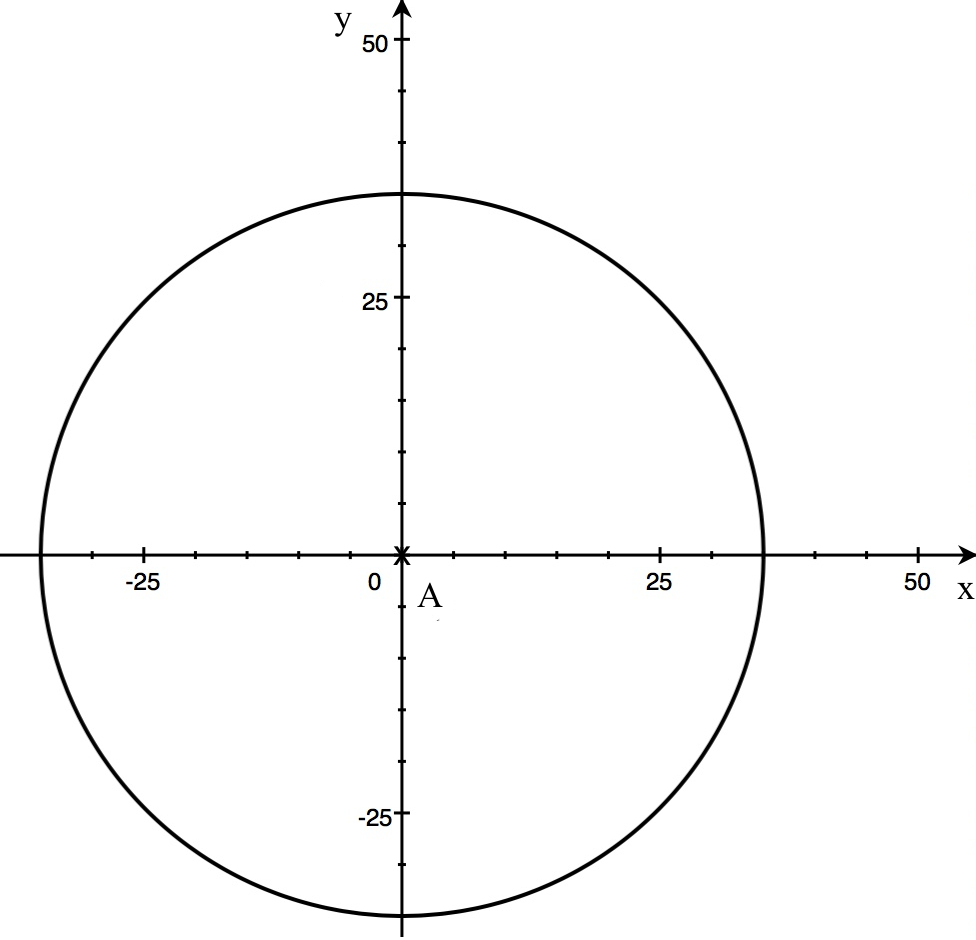
\includegraphics[width=12cm]{dia1.png}
	\caption{Kreisbewegung mit Mittelpunkt bei A(0\big|0)}
\end{figure}\\
Das Problem ist nun, dass die Pixel eines Bildes nur positive Koordinaten haben. Dies lässt sich dadurch korrigieren, dass man zu den x-Koordinaten die Hälfte der Breite des Bildes und zu den y-Koordinaten die Hälfte der Höhe des Bildes addiert:
\begin{align}
x &= \cos (\alpha) \cdot r + \frac{Breite \ des \ Bildes}{2} \\
y &= \sin (\alpha) \cdot r +  \frac{\text{Höhe\ des\ Bildes}}{2}
\end{align}
Wir addieren die Hälfte der Höhe des Bildes und die Hälfte der Breite des Bildes, da dies die Mindestgröße ist, damit sich der Graph im ersten Quadranten befindet. Dadurch verändert sich der Mittelpunkt, wie auf Abb. 2 zu sehen ist, auf den Punkt M(35\big|35).
\begin{figure}[h]
	\centering
	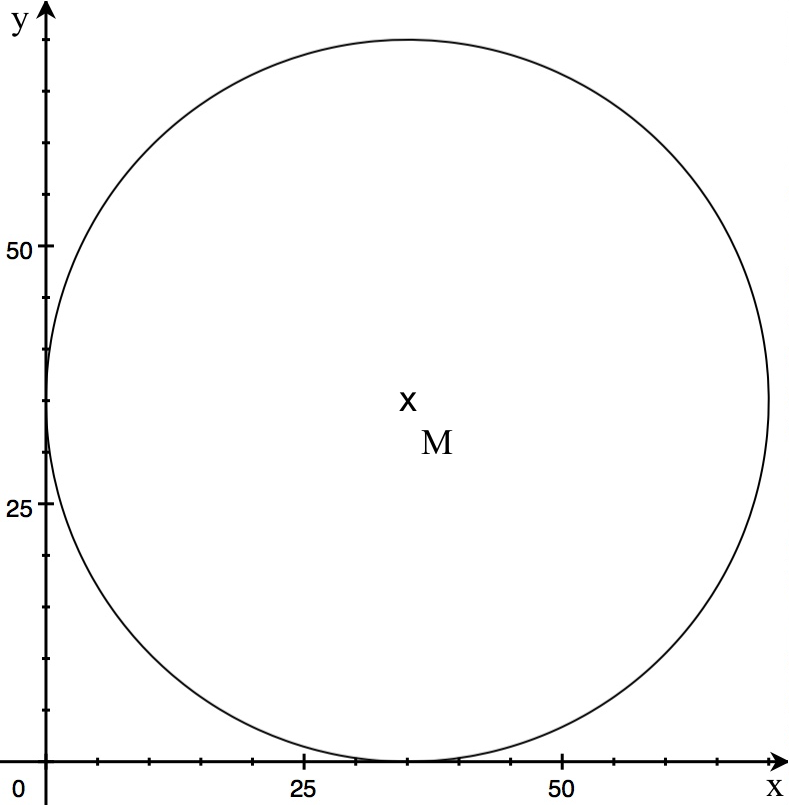
\includegraphics[width=12cm]{dia2.png}
	\caption{Kreisbewegung mit Mittelpunkt bei M(35\big|35)}
\end{figure}\\
\\Diese physikalischen Aspekte haben wir in unserem Programm folgendermaßen umgesetzt:
\subsection{Welche Mindestgeschwindigkeit wird gebraucht?}
Das menschliche Auge nimmt Bilder in einer Frequenz f\textsubscript{Auge} von 10 bis 12Hz auf\textsuperscript{17}. Um die Geschwindigkeit bei rund 10Hz zu berechnen, verwenden wir die Formel $v = \frac{\Delta s}{\Delta t}$. Auf die Kreisbewegung angewandt entspr"ache dies $v = \frac{2\pi r}{T}$ in $\frac{m}{s}$. Da $\frac{1}{T}$ der Frequenz entspricht, der Umrechnungsfaktor von $\frac{m}{s}$ in $\frac{km}{h}$ 3,6 ist und $d = 2 \cdot r$ gilt, erhalten wir die Formel $v = \pi \cdot f\textsubscript{Auge} \cdot d \cdot 3,6$. Durch das Anbringen der vier Streifen am Rad, ben"otigen wir nur ein viertel der urspr"ungliche Geschwindigkeit. Demnach gilt: 
\begin{align}
v = \frac{\pi \cdot f\textsubscript{Auge} \cdot d \cdot 3,6}{4}
\end{align}
Also beträgt die Mindestgeschwindigkeit rund $v \approx 17\frac{km}{h}$ bei einem 24\grqq\ Rad, um ein vollständiges Bild zu erkennen. Die Geschwindigkeit, bei der schon ein Bild zu erkennen ist, ist jedoch kleiner, weil das Gehirn ein Bild selbst vervollständigt. Dem Gehirn genügt es, einige Konturen wahrzunehmen, um ein Bild oder Objekt zu erkennen, da es den Rest aus Erfahrung und Fantasie ergänzt\textsuperscript{18}.
\subsection{Ansteuerung des Led Streifens}
Der verwendete LED-Streifen hat die Mod so werden diese an die zweite LED übertragen, die wiederum nur die ersten 24bit für sich selbst übernimmt und den Rest weiterschickt usw.. ellnummer ws2812b und wird wie folgt angesteuert\textsuperscript{[19]}:
Jede Led des LED-Streifens wird durch ein 24bit Signal angesteuert, das mittels Pulsweitenmodulation vom Raspberry Pi auf diesen übertragen wird. Die Farbanteile Grün, Rot und Blau werden je über acht bit angesteuert, so dass man pro pixel 2\textsuperscript 8 also 256 und mit allen drei LEDs 16.777.216 verschiedene Farben anzeigen kann. Die Reihenfolge der Farbansteuerung ist in folgendem Diagramm verdeutlicht:
\begin{figure}[h]
	\centering
	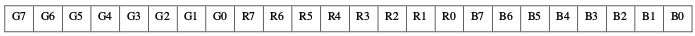
\includegraphics[width=17cm]{AufbauDer24BitAnsteuerungDesStreifens.png}
	\caption{Reihenfolge der Bits bei der Ansteuerung einer LED des LED-streifens}
\end{figure}\\
Falls nach diesem 24Bit Signal, innerhalb der Taktung\textsuperscript{[19]} noch weitere Signale an den LED-Streifen übertragen werden, so werden diese über den DOUT(siehe Abbildung 4) anschluss an die zweite LED übertragen, die wiederum nur die ersten 24bit für sich selbst übernimmt und den Rest weiterschickt usw.. 
\begin{figure}[h]
	\centering
	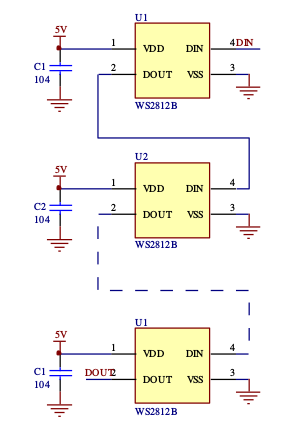
\includegraphics[width=5cm]{Schaltplan_des_LED-Streifens.png}
	\caption{Schaltplan des Led-streifens\textsuperscript{[19]}}
\end{figure}

\subsection{Programm}
Wir haben das Programm in Python 3 geschrieben. Zu Beginn haben wir uns hauptsächlich an dem Programm strandtest.py orientiert, welches in der Adafruit-Neopixel-Library\textsuperscript{3} enthalten ist. Dieses Programm beinhaltete die Abfolge verschiedener Farben, die der LED- Streifen anzeigt. Anhand dieses Programms konnten wir die Reihenfolge und Darstellung der Farbwerte erschließen, welche in diesem Fall GRB ist.
\subsubsection{Programmabschnitt 1}
In unserem fertigen Programm importieren wir anfangs die Module time, math und RPi.GPIO und die Libraries neopixel und PIL, welche wir für das später gebrauchen werden. Daraufhin haben wir verschiedene Variablen definiert, welche das Bild mittels der Funktion \textcolor{blue}{$open$}{$()$} der PIL öffnen, es mit der Funktion {$im.$}\textcolor{blue}{$load$}{$()$} laden und uns die Breite und Höhe des Bildes mit {$im.$}\textcolor{blue}{$size$}{$()$} ausgeben. Wie man im Prog. 4 später sieht ist es egal, ob das Bild RGB-Werte oder CMYK-Werte besitzt. Um das kommende Program effizienter zu gestallten, haben wir hier schon {$breite$} und {$h\text{ö}he$} als die Hälfte der Breite des Bildes und die Hälfte der Höhe des Bildes definiert. Die im Program benötigten Größen, die Anzahl der LEDs, die Nummer des Pins, der den LED-Streifen ansteuert, die Nummer des Pins, der den Magnetschalter ansteuert, die Frequenz der LEDs, der DMA-Kanal, die Helligkeit und die Anzahl der Streifen, werden daraufhin alle definiert. Zusätzlich haben wir diverse Variablen definiert, welche wir für numerische Schleifen oder zum späteren Definieren benötigen.
\begin{figure}[h]
	\centering
	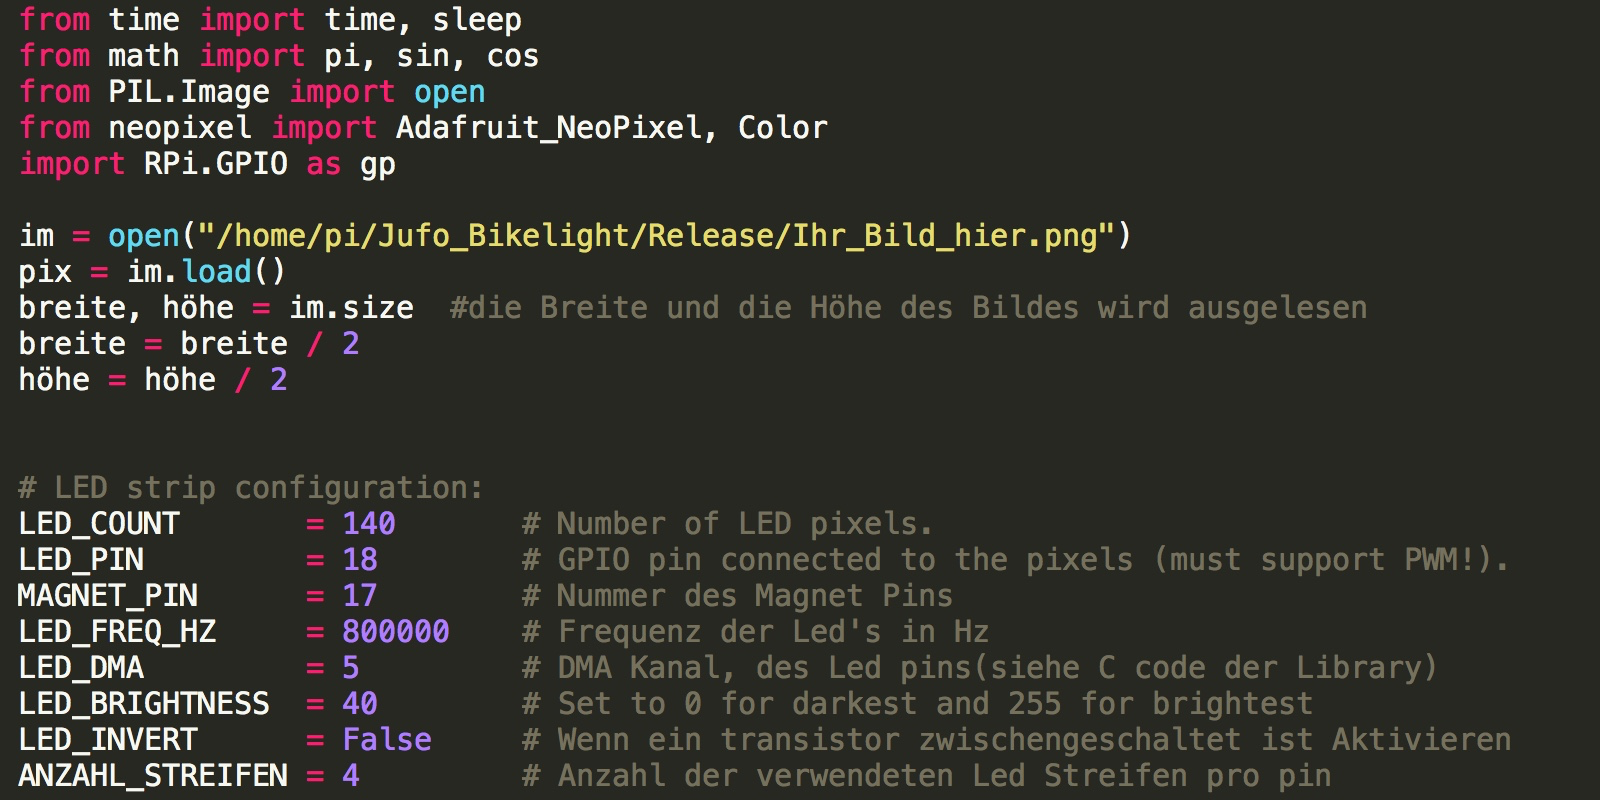
\includegraphics[width=16cm]{P1.png}
	\caption{Programmabschnitt 1}
\end{figure}
\subsubsection{Programmabschnitt 2}
Danach erschaffen wir die Liste {$radien$}, in der wir \textcolor{violet}{$0$} fünfunddreißigmal mit einer numerischen Schleife, die wir mittels der Funktion \textcolor{blue}{$range$}{$()$} mit der Untergrenze \textcolor{violet}{$0$} und der Obergrenze, die der Quotient aus LED\_COUNT und ANZAHL\_STREIFEN ist, erschaffen, einfügen, da man nicht solch eine Liste in der zweiten numerischen Schleife erschaffen kann, inder man die Radien als einzelne Werte in die Liste einfügt. Der Datentyp des Quotienten ist ein Float. Da die Funktion \textcolor{blue}{$range$}{$()$} nur mit Integer arbeitet, ändern wir den Typen des Quotienten mittels der Funktion \textcolor{blue}{$int$}{$()$} zu einem Integer. Danach erstellen wir eine weitere numerische Schleife für {$i$} (siehe Prog. 1) und denselben Grenzen und erschaffen damit die Radien. Wir ersetzen die \textcolor{violet}{$0$} an {$i$}-ter Stelle durch die Summe aus {$i$}, \textcolor{violet}{$1$}, und der Variablen {$minR$}. Die Addition von \textcolor{violet}{$1$} ist notwendig, da die Aufzählung sonst bei \textcolor{violet}{$0$} begänne. Die Addition von {$minR$} ist nötig, da wir die ersten fünf Radien nicht verwenden können, weil sich dort aufgrund der Radnabe keine LEDs befinden. 
Da wir {$i$} im Bereich von 0 bis 35 aufzählen, decken wir alle 35 Radien ab, die zuerst \textcolor{violet}{$0$} waren und dann ersetzt werden. Wir haben 35 Radien, da ein Teilstreifen 35 LEDs besitzt.
\begin{figure}[h]
	\centering
	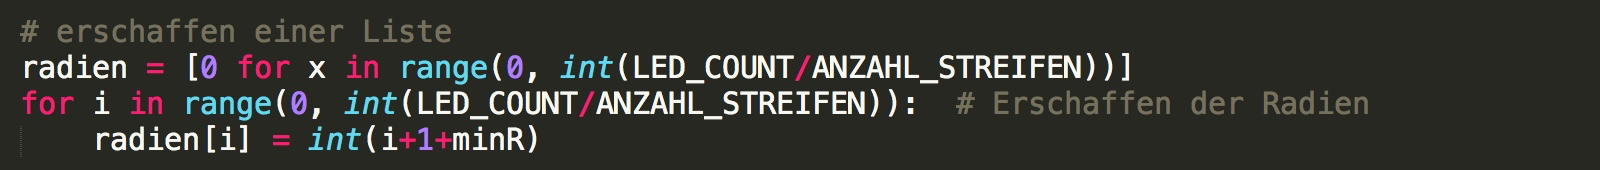
\includegraphics[width=16cm]{P2.png}
	\caption{Programmabschnitt 2}
\end{figure}
\newpage
\subsubsection{Programmabschnitt 3}
Die zwei Funktionen \textcolor{green}{$line$}{$()$} und \textcolor{green}{$startPrint$}{$()$} beziehen sich auf die Herstellung der Startanzeige.
Die Funktion \textcolor{green}{$line$} erstellt die Abgrenzungen der Startanzeige. Anfangs wird ein leerer String {$s$} erzeugt. Dieser String erhält dann mit einer numerischen Schleife für {$i$} (siehe Prog. 1) in dem Bereich von \textcolor{violet}{$0$} bis \textcolor{orange}{$l\text{ä}nge$}, welcher in der Funktion startPrint{$()$} gewählt wird, Striche (je nachdem wie \textcolor{orange}{$l\text{ä}nge$} gewählt wird) und wird am Ende der Funktion ausgegeben. Die Funktion \textcolor{green}{$startPrint$}{$()$} gibt die Startanweisung aus. In der Startanweisung werden die wichtigsten Größen für den Benutzter ausgegeben. Als Parameter für die Funktion \textcolor{green}{$line$}{$()$} haben wir \textcolor{violet}{$50$} gewählt, da dies eine geeignete Länge für eine Abgrenzung ist. am Ende wird die Ausgabe erzeugt, dass man das Programm mittels der Tastenkombination Strg-c beenden kann.
\begin{figure}[h]
	\centering
	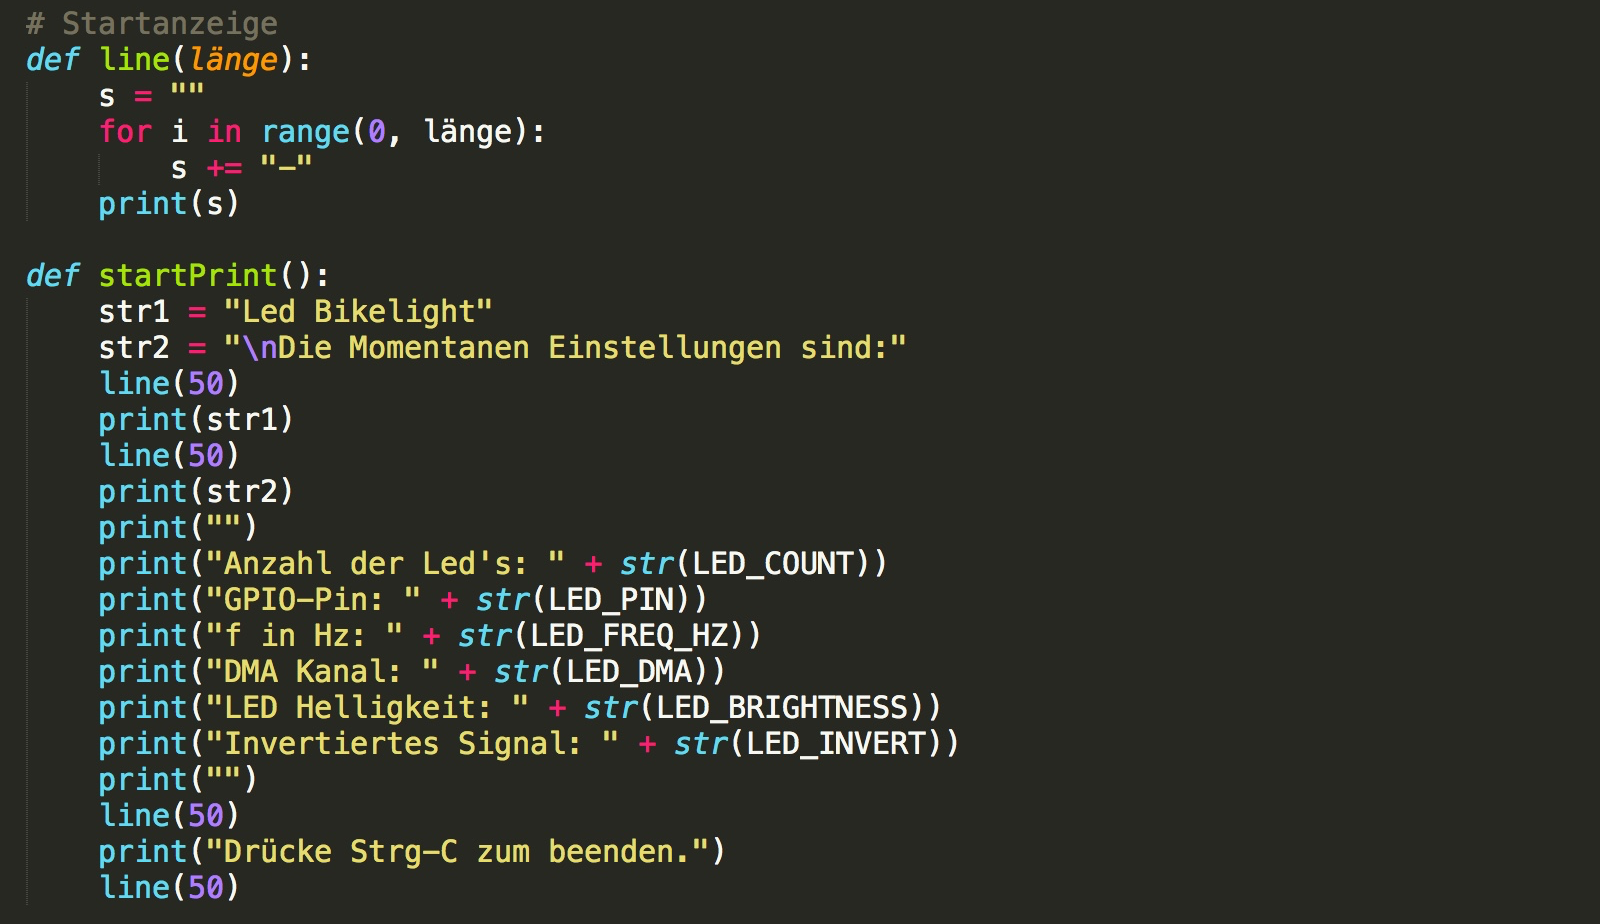
\includegraphics[width=16cm]{P3.png}
	\caption{Programmabschnitt 3}
\end{figure}
\begin{figure}[h]
	\centering
	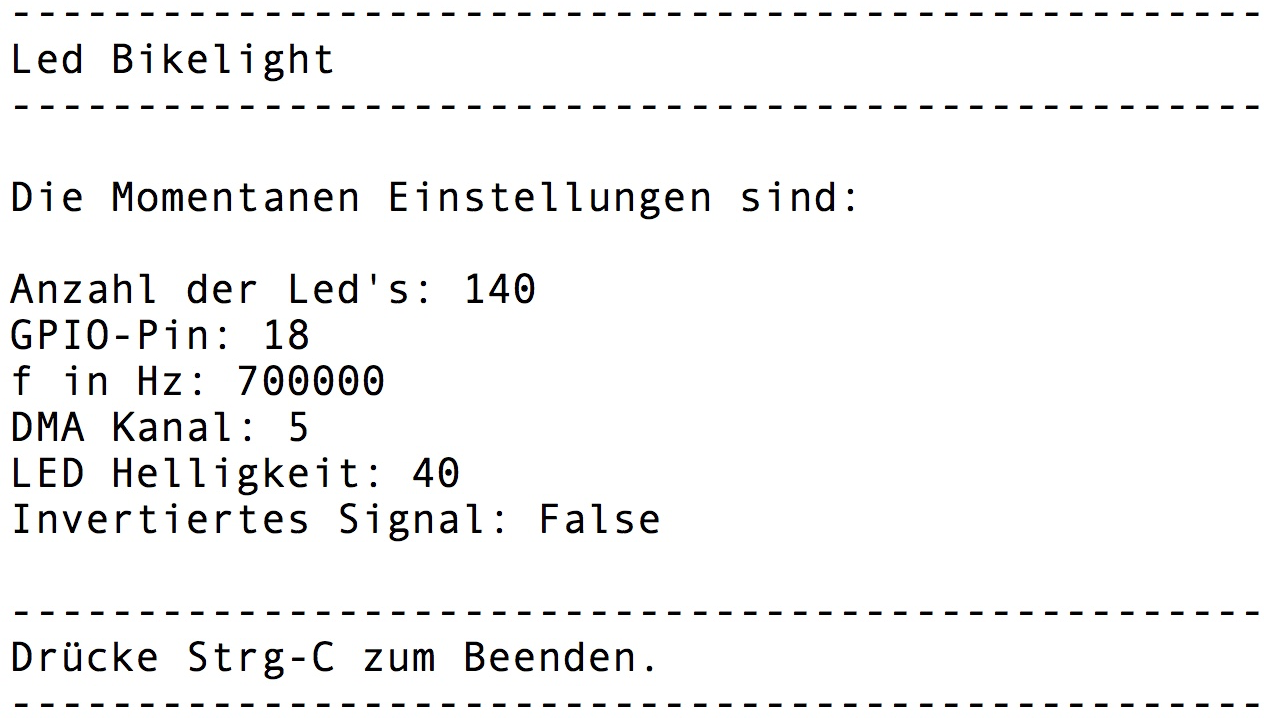
\includegraphics[width=8cm]{Startanzeige.png}
	\caption{Startanzeige}
\end{figure}
\subsubsection{Programmabschnitt 4}
Die Funktion \textcolor{green}{$bildAuslesen$}{$()$} gibt zu jeder Position der LEDs die x- und y-Koordinaten und die dazugehörigen RGB-Werte im Bild aus. Die x- und die y-Koordinate werden mit den Formeln 7 und 8 (siehe Physikalische Beschreibung) berechnet. Da die Funktionen \textcolor{blue}{$sin$}{$()$} und \textcolor{blue}{$cos$}{$()$} auf fünfzehn Stellen genau die Koordinaten ausgegeben, wir sie allerdings nur mit einer Dezimalstelle genau benötigen, werden die Formeln 7 und 8 folgendermaßen geändert:
\begin{align}
x \approx \cos (\alpha) \cdot r + \frac{\text{Breite \ des \ Bildes}}{2} \\
y \approx\sin (\alpha) \cdot r + \frac{\text{Höhe\ des\ Bildes}}{2}
\end{align}
Im Programm runden wir sie mit der Funktion \textcolor{blue}{$round$}{$()$} auf die erste Dezimalstelle. Danach werden die RGB Werte an den Koordinaten x und y mit der Funktion pix[x, y] (siehe Prog. 1) ausgelesen. Mit Hilfe einer try-except-Anweisung kann unser Programm zwischen Bildern mit RGB-Werten oder CMYK-Werten unterscheiden und mit der Anweisung \textcolor{red}{$return$} \textcolor{blue}{$Color$}(g, r, b) beziehngsweise \textcolor{red}{$return$} \textcolor{blue}{$Color$}(g, r, b, \_) an den LED- Streifen übergeben. Bei der Variante mit den CMYK-Werten lassen wir die Schwarzwerte raus, da wir sie nicht benötigen. Dies geschieht in der Reihenfolge g, r, b (siehe Prog. 1).
\begin{figure}[h]
	\centering
	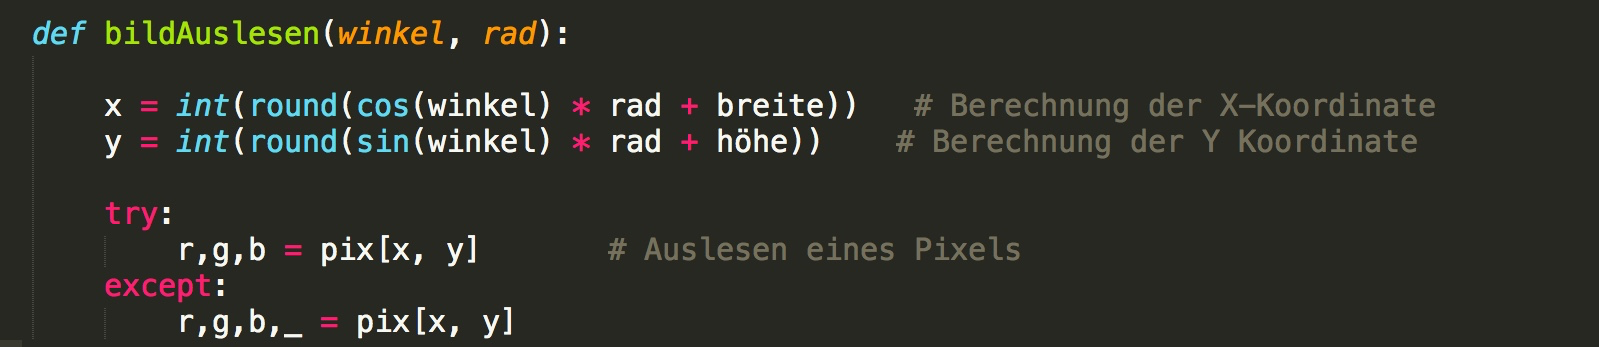
\includegraphics[width=16cm]{P4.png}
	\caption{Programmabschnitt 4}
\end{figure}
\subsubsection{Programmabschnitt 5}
In der Funktion \textcolor{green}{$streifenBedienen$}{$()$} werden zuerst die Liste mit den Radien {$radien$}, der LED-Streifen {$streifen$} (siehe Prog. 6) und die im ersten Programmabschnitt voreingestellte Umlaufzeit {$T$}, Zeitabschnitt {$t$} und Winkelgeschwindigkeit \textomega\ globalisiert, da wir diese über mehrere Funktionen benötigen und die Globalisierung effizienter ist, als sie als Parameter zu übergeben. Die Winkel alpha, beta, gamma und delta werden nach Formel 4 berechnet. Die Winkelgeschwindigkeit und der Zeitabschnitt werden jedoch in \textcolor{green}{$main$}{$()$} berechnet. Da die LED-Streifen in einem Winkel von 90$^\circ$ gedreht sind (siehe Anhang Abb. 3), addieren wir zum vorhin berechneten Winkel 90$^\circ$ beziehungsweise
$\frac{\pi}{2}$
hinzu. Weil der Zeitabschnitt {$t$} größer wird, wachsen die Winkel an, was die Bewegung der LEDs im Bild simuliert. Dann haben wir {$n$} als Anzahl der Pixel des LED-Streifens, {$u$} als Anzahl der Pixel auf einen Teilstreifen und {$M$} als die Hälfte der Anzahl der Pixel des LED-Streifens definiert. Die erste numerische Schleife zählt bis {$u$} hoch, dabei wird {$i$} um 1 erweitert und {$u$}  um 1 verringert. Die Funktion \textcolor{green}{$bildAuslesen$}{$()$} ermittelt dann für den ersten und dritten Streifen (siehe Anhang Abb. 3) die RGB-Werte. Wir lassen die Radien rückwärts von der Liste {$radien$} aufzählen, indem wir {$u = u - 1$} rechnen. Demnach nimmt bei größer werdendem {$i$} {$u$} von 35 bis 0 ab und in dieser Reihenfolge werden die Radien aus der Liste {$radien$} aufgerufen. Die Radien müssen rückwärts aufgerufen werden, da die PIL das Bild vom Zentrum aus ausliest, der erste und dritte LED-Streifen jedoch von außen angeschlossen sind (siehe Anhang Abb. 3). Da {$u$} in der ersten numerischen Schleife heruntergezählt wurde, mussten wir {$u$} nochmals definieren. Die RGB-Werte werden mit der Nummer der jeweiligen LED der Funktion {$streifen.$}\textcolor{blue}{$setPixelColor$}{$()$} übergeben. Wir erhalten für den ersten Streifen die richtige Reihenfolge, da {$i$} von 0 bis 35 aufgezählt wird und für den dritten Streifen ebenfalls, weil wir {$i$} mit {$M$} addieren, weil der dritte Streifen einen halben Streifen vom ersten entfernt ist. Die zweite numerische Schleife zählt von {$u$} bis {$M$}. Die Funktion \textcolor{green}{$bildAuslesen$}{$()$} gibt die RGB-Werte des zweiten und vierten LED-Streifens an. Die Radien werden diesmal in der richtigen Reihenfolge aus der Liste entnommen, da diese LED-Streifen von innen angeschlossen sind (siehe Anhang Abb. 3). Anschließend werden die RGB-Werte zusammen mit der Nummer der anzustauenden LED an die Funktion {$streifen.$}\textcolor{blue}{$setPixelColor$}{$()$} übergeben. Die Nummerierung der LEDs am zweiten Streifen verläuft von 35 bis 70, da {$i$} in der numerischen Schleife hochgezählt wird. Die Nummerierung der LEDs am vierten Streifen geht von 105 bis 140, weil der Streifen 70 LEDs vom zweiten Streifen entfernt war. Diese Aufzählung erreicht man, indem man {$i$} mit {$M$} addiert. Am Ende von \textcolor{green}{$streifenBedienen$}{$()$} bringt die Funktion {$streifen.$}\textcolor{blue}{$show$}{$()$} die LED-Streifen zum Leuchten.
\begin{figure}[h]
	\centering
	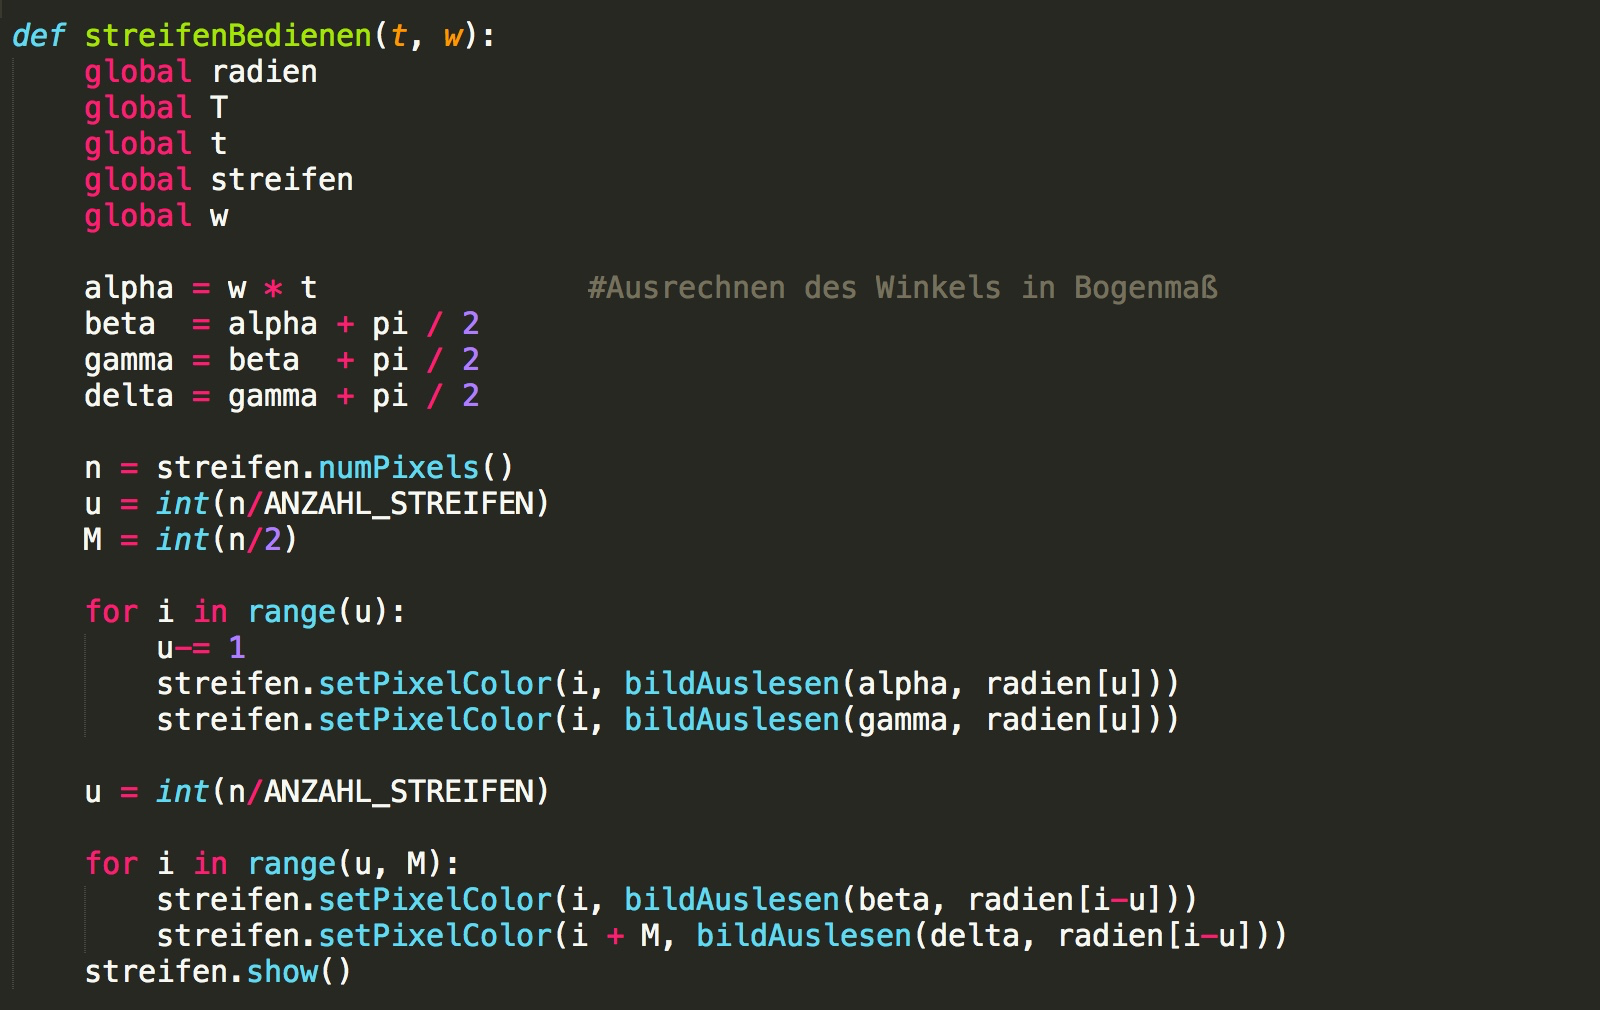
\includegraphics[width=16cm]{P5.png}
	\caption{Programmabschnitt 5}
\end{figure} 
\subsubsection{Programmabschnitt 6}
In der Funktion \textcolor{green}{$main$}{$()$} werden zuerst die benötigten Variablen globalisiert. Dies sind die Umlaufzeit {$T$}, der Zeitabschnitt {$t$}, die Zeit seit dem Beginn der Umdrehung {$t1$}, die Liste {$radien$} mit den Radien, der LED-Streifen {$streifen$} und die Winkelgeschwindigkeit \textomega. Danach wird mit der Anweisung {$gp.$}\textcolor{blue}{$setmode$}{$(gp.BCM)$} festgelegt, dass GPIO-Nummern verwendet werden. Mit der Anweisung {$gp.$}\textcolor{blue}{$setwarnings$}{$($}\textcolor{violet}{False}{$)$} wird festgelegt, dass keine Warnungen ausgegeben werden, da wir diese nicht benötigen und mit der Anweisung {$gp.$}\textcolor{blue}{$setmode$}{$(MAGNET\_PIN, gp.IN)$} wird {$MAGNET\_PIN$} (siehe ersten Programmabschnitt) als Eingang festgelegt. Mit der Methode {$Adafruit\_NeoPixel$} wird mit den Eigenschaften {$LED\_COUNT, LED\_PIN, LED\_FREQ\\ \_HZ, LED\_DMA, LED\_INVERT, LED\_BRIGHTNESS$} das Objekt {$streifen$}, also der LED-Streifen erstellt. Die Funktion {$streifen.$}\textcolor{blue}{$begin$}{$()$} initialisiert den LED-Streifen und die Funktion \textcolor{blue}{$startPrint$}{$()$} gibt die Startanzeige aus. In der darauf folgenden while-Schleife wird festgelegt, dass die Zeit seit dem Beginn der Umdrehung gleich der Systemzeit ist. Danach wird die Bedingung formuliert, dass, falls der Magnetschalter {$MAGNET\_PIN$} nicht auslöst, die Winkelgeschwindigkeit \textomega\ mit der Formel 2 berechnet wird. In dieser if-Anweisung befindet sich eine while-Schleife, welche auslöst, wenn der Magnetschalter nicht auslöst. In dieser while-Schleife wird ein Zeitabschnitt berechnet und da diese while-Schleife mehrere male auslöst werden mehrere Zeitabschnitte berechnet, die man für die Winkelberechnung benötigt (siehe Prog. 5). Ebenfalls wird die Funktion streifenBedienen{$()$} aufgerufen, welche den LED-Streifen dann zum Leuchten bringt. Wenn der Magnetschalter auslöst, also die if-Anweisung nicht zutrifft, wird die Umlaufzeit nach der Formel 1 berechnet. Da wir anfangs (siehe Prog. 1) {$T$} und {$t$} definiert haben, erhalten wir \textcolor{red}{$UnboundLocalError$} nicht.
\begin{figure}[h]
	\centering
	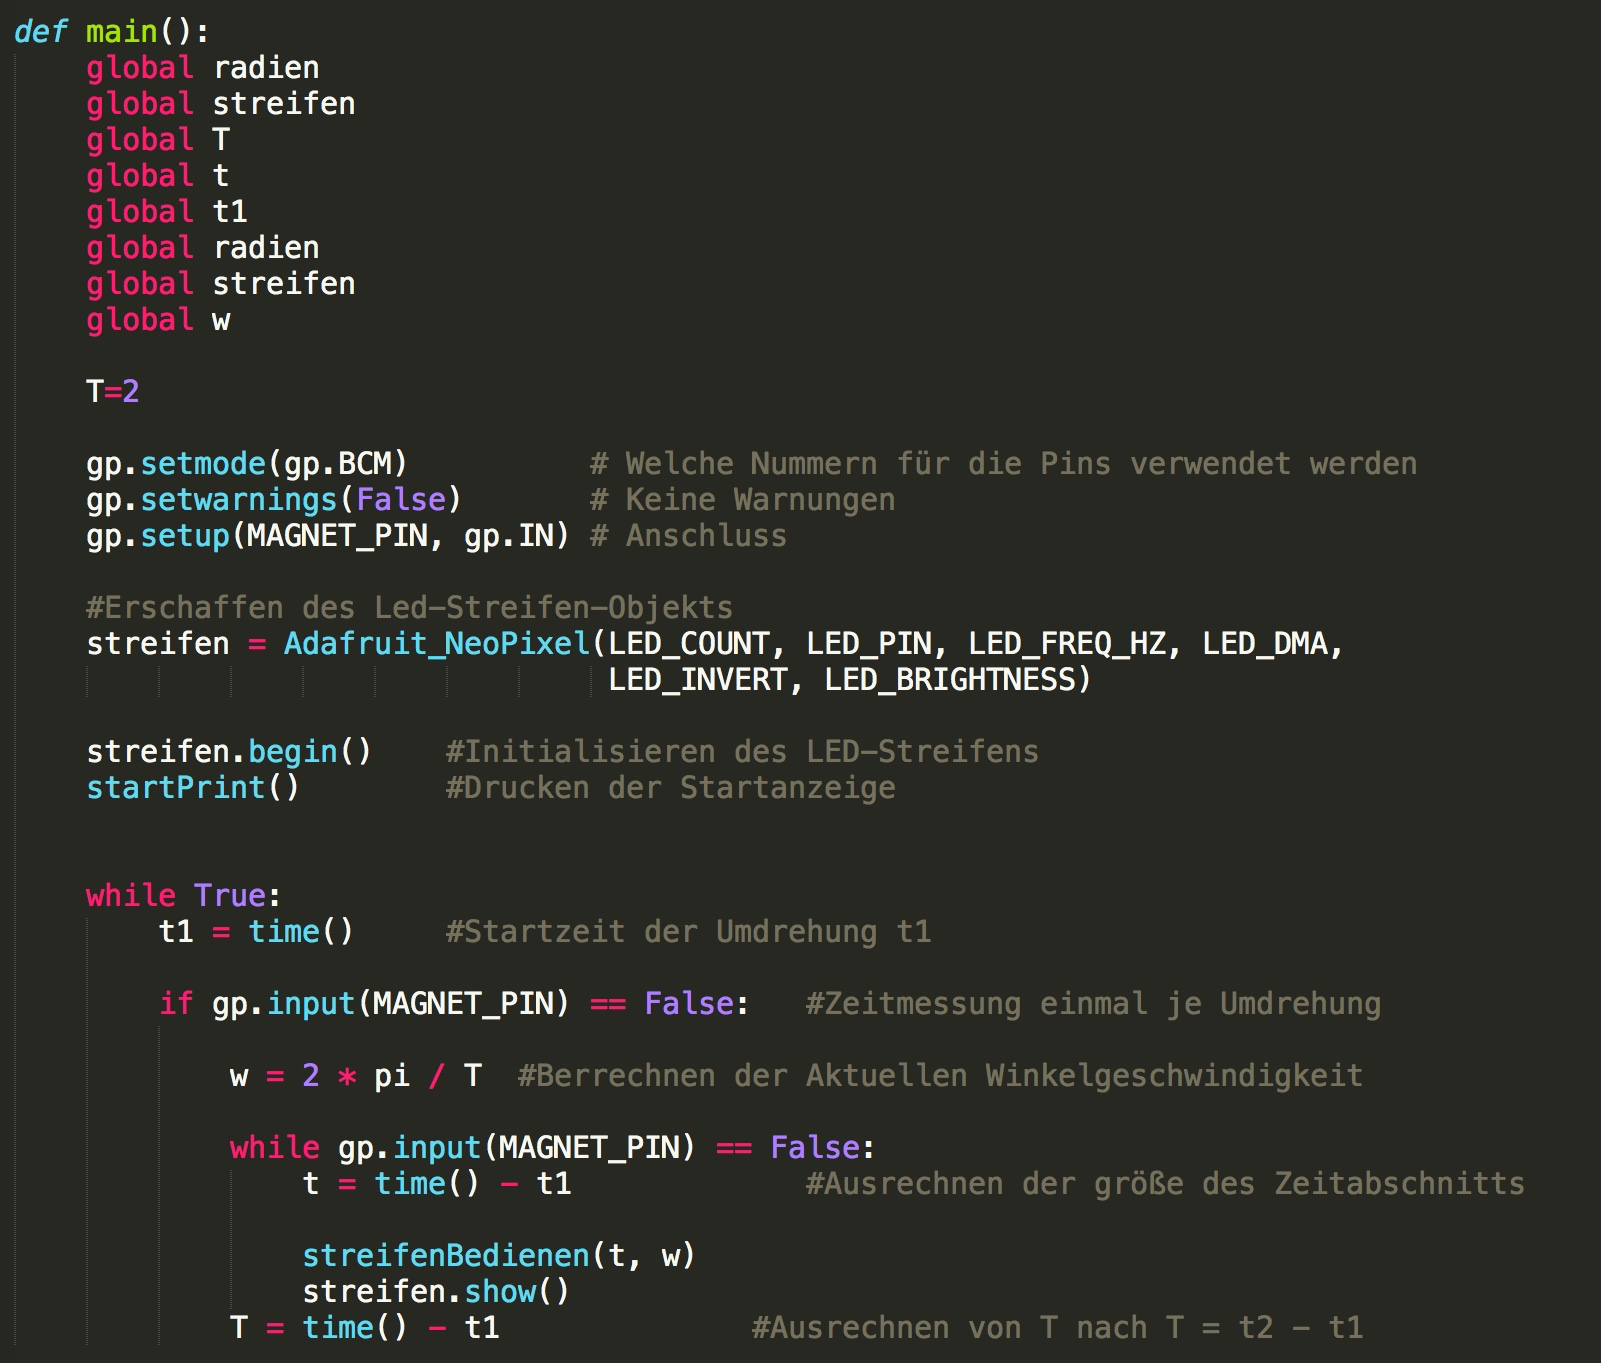
\includegraphics[width=16cm]{P6.png}
	\caption{Programmabschnitt 6}
\end{figure} 
\subsubsection{Programmabschnitt 7}
Die Funktion \textcolor{blue}{$main$}{$()$} wird aufgerufen, indem eine if-Anweisung auslöst, wenn der Name des Programms {$main$} ist, was hier der Fall ist.
\begin{figure}[h]
	\centering
	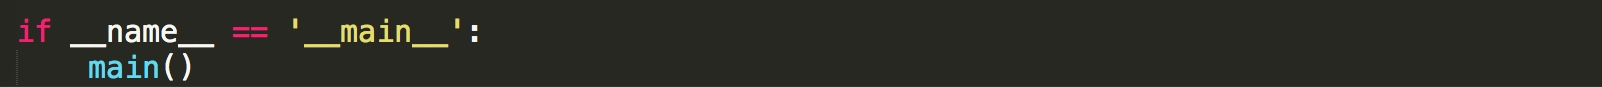
\includegraphics[width=16cm]{P7.png}
	\caption{Programmabschnitt 7}
\end{figure}
\subsection{Aufbau und Montage}
\subsubsection{Installation des Raspberry Pi{'}s}
Als erstes haben wir eine microSD-Karte mit dem Betriebssystem Raspbian\textsuperscript{6}\ bespielt und haben einen WLAN-USB-Stick von seinem Gehäuse entnommen und nach einem Bild\textsuperscript{7} mit dem Raspberry Pi Zero verbunden. Danach haben wir die SD-Karte in einen Computer gesteckt und haben in die Datei {$/etc/wpa\_supplicant/wpa\_supplicant.conf$} Netzwerkdetails hinzugefügt\textsuperscript{8}.
Danach haben wir den Raspberry Pi an einen Monitor angeschlossen, ihn zum ersten mal gebootet und mit Hilfe des Befehls {$raspi-config$}\textsuperscript{9}\ den Zugriff auf den Raspberry Pi durch SSH ermöglicht. Seinen Hostnamen haben wir zu Spokescreen geändert. Danach konnten wir über jeden PC in unserem Heimnetzwerk, auf welchem ein SSH-Client installiert war, auf das Terminal des Raspberry Pis zugreifen.
Nun haben wir git, den Github Client für Linux, auf dem Raspberry Pi installiert und unser Github Repository\textsuperscript{10}\ auf den Pi mit dem Befehl {$git\ clone\ https://github.com/ RubenHaag/Jufo\_Spokescreen$} heruntergeladen. Danach haben wir die Python Image Library\textsuperscript{5}, zum Auslesen eines Bildes mit Python, und die Adafruit Neopixel Library\textsuperscript{3}, zum Ansteuern der LED-Streifen installiert. Um nun unsere LED-Streifen zu testen, haben wir uns zuerst einen Schaltplan mit Hilfe des Tools Fritzing\textsuperscript{11} gezeichnet.\\
\begin{figure}[h]
	\centering
	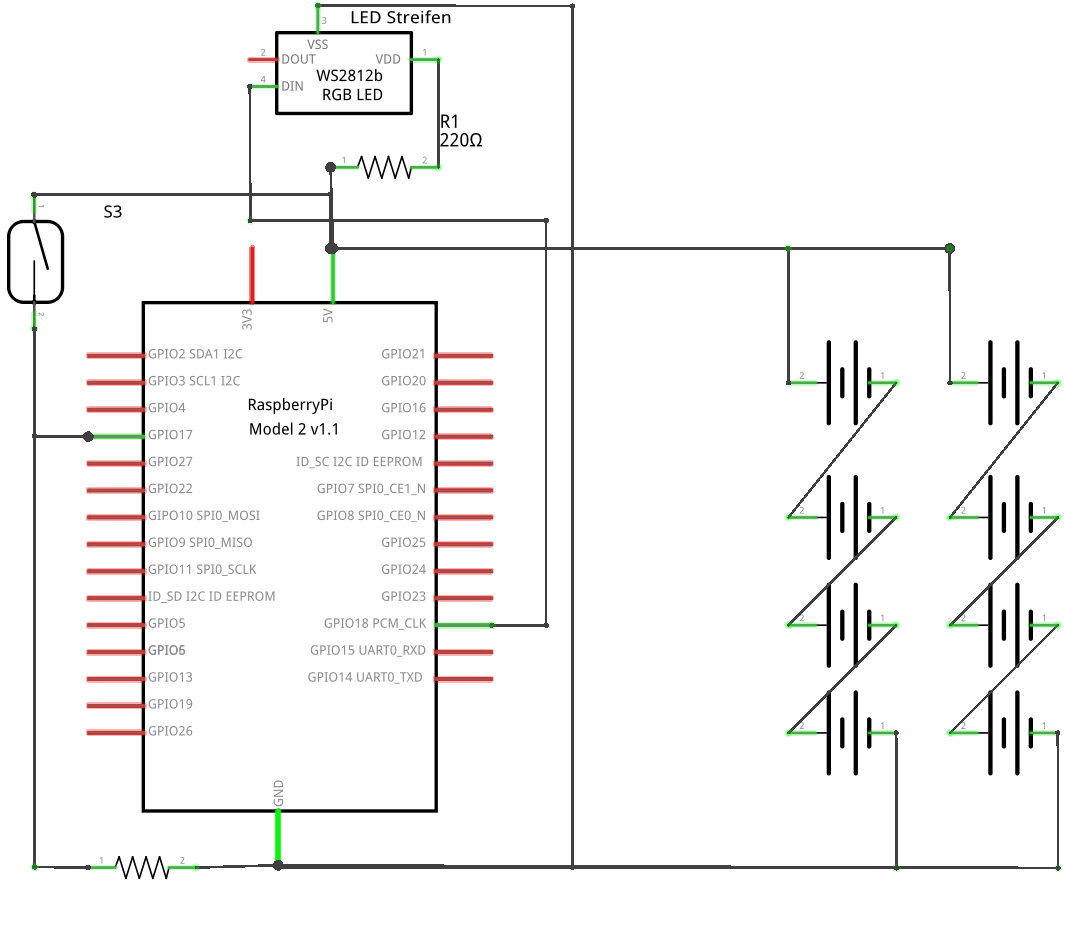
\includegraphics[width=10cm]{u.png}
	\caption{Schaltplan}
\end{figure}
\\
Der Raspberry Pi ist mit einem seiner Ground-Pins mit der Masse verbunden und mit einem der beiden 5-Volt-Pins direkt mit der Spannungsquelle verbunden. Der LED Streifen ist ebenfalls mit dem 5-Volt- und Ground-Pin verbunden und wird über den GPIO-18-Pin des Raspberry Pis angesteuert, da dieser als einer der wenigen die für die Ansteuerung des Streifens essentielle Pulsweitenmodulation (PWM) unterstützt. Um die Zeit nun einmal pro Umdrehung zu messen, verwenden wir das Reed-Relais (Magnetschalter) eines Fahrradtachos. Durch diese Relais fließt, wenn er in die Nähe des an der Gabel befestigten Magneten kommt, Strom, da sich die Kontakte im Relais schließen, welcher über den GPIO-17-Pin des Raspberry Pis ausgelesen wird. Zur Absicherung des Raspberry Pis gegen eventuelle Spannungsschwankungen ist der Magnetschalter zusätzlich noch über einen Widerstand von 7M\textOmega\ mit dem Ground-Pin verbunden. Die Stromversorgung liefern zwei USB-Powerbanks mit je 5000 mAh. Sie liefern eine konstante Spannung von je 5 V, besitzen eine relativ hohe Energiedichte und sind trotzdem vergleichsweise leicht. Diese sind parallel geschaltet, damit die Spannung den Raspberry Pi nicht überlastet, und stellen die Stromversorgung mit 5 V dar. Die Powerbanks haben wir angeschlossen, indem wir zwei USB Kabel abisoliert und mit Standard-Pin-Anschlüssen versehen haben (Polung siehe Lit. [4]). Diesen Schaltplan haben wir zuerst auf einem Breadboard zusammengebaut, um zu testen, ob die LED-Streifen und der Magnetschalter funktionieren. Als einen ersten Test für den LED- Streifen haben wir das bei der Adafruit NeoPixel Library\textsuperscript{3} mitgelieferte Programm \glqq Strandtest.py\grqq\ verwendet.
\subsubsection{Aufbau und Funktion des ersten Tests mit dem LED-Streifen}
Für den Magnetschalter haben wir ein Programm geschrieben, um die Zeit zwischen zwei Signalen von diesem zu messen (siehe Programm).
Da alle Komponenten ohne Probleme funktionierten, haben wir nun den LED-Streifen in vier Teile á 36 LEDs geteilt und für einen größeren Spielraum haben wir von jedem Streifen eine LED entfernt. Zuerst haben wir versucht, die vier unterschiedlichen LED-Streifen an vier unterschiedlichen GPIO-Pins anzuschließen, bis wir festgestellten, dass der verwendete Raspberry Pi 3 und der Raspberry Pi Zero, den wir später anschließen wollten, nur 6 GPIO-Pins haben, die PWM unterstützen. Um auf jeder Seite vier LED-Streifen anzubringen, hätten wir jedoch mindestens 8 Pins benötigt, also haben wir die vier LED-Streifen in Reihe geschaltet und so nur den PWM fähigen GPIO-18-Pin verwendet.
Daraufhin haben wir den Schaltplan auf eine Platine übertragen und die vier LED-Streifen durch unterschiedlich lange Kabelstücke miteinander verbunden, um sie später entsprechend auf dem Reifen zu platzieren. Die Platine haben wir nun in eine wasserdichte Verteilerbox eingebaut und mit Kabelbindern an den Speichen befestigt.
Nach ersten misslungenen Versuchen mit Kunststoffhalterungen haben wir uns aus Stabilitätsgründen für eine Märklin-Metall-Halterung entschieden, um die Elektronik sicher an dem Speichenrad zu befestigen. Die Halterung haben wir um die Nabe herum in einem rechtwinkligen Kreuz angeordnet. Dann haben wir die LED-Streifen auf feste Kunststoffstreifen geklebt und diese dann mit Kabelbindern an dem Metallkreuz befestigt. Dieses wurde wiederum an einer Fahrradgabel montiert und fixiert. Dann haben wir die Felge über einen Märklin Metall-Motor angetrieben, um eine gleichbleibende, einstellbare Geschwindigkeit zu erhalten, die der Geschwindigkeit eines durchschnittlichen Fahrradfahrers entspricht. Der finale Aufbau ist in Abb. 14 dargestellt:
\begin{figure}[h]
	\centering
	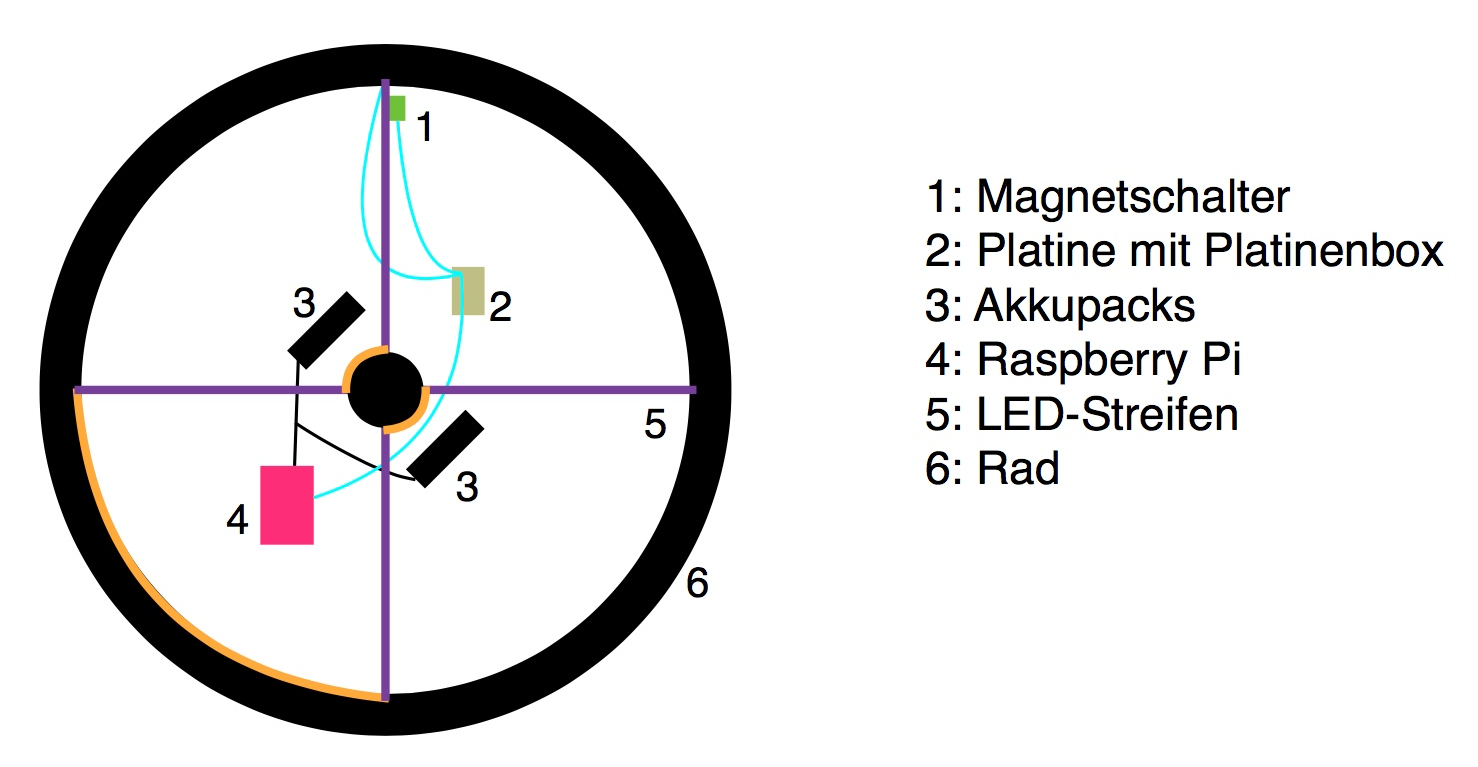
\includegraphics[width=9.5cm]{Rad.png}
	\caption{Skizze des Aufbaus}
\end{figure}
\subsection{Welche Mindestgeschwindigkeit wird gebraucht?}
Das menschliche Auge nimmt Bilder in einer Frequenz f\textsubscript{Auge} von 10 bis 12Hz auf\textsuperscript{17}. Um die Geschwindigkeit bei rund 10Hz zu berechnen, verwenden wir die Formel $v = \frac{\Delta s}{\Delta t}$. Auf die Kreisbewegung angewandt entspr"ache dies $v = \frac{2\pi r}{T}$ in $\frac{m}{s}$. Da $\frac{1}{T}$ der Frequenz entspricht, der Umrechnungsfaktor von $\frac{m}{s}$ in $\frac{km}{h}$ 3,6 ist und $d = 2 \cdot r$ gilt, erhalten wir die Formel $v = \pi \cdot f\textsubscript{Auge} \cdot d \cdot 3,6$. Durch das Anbringen der vier Streifen am Rad, ben"otigen wir nur ein viertel der urspr"ungliche Geschwindigkeit. Demnach gilt: 
\begin{align}
v = \frac{\pi \cdot f\textsubscript{Auge} \cdot d \cdot 3,6}{4}
\end{align}
Also beträgt die Mindestgeschwindigkeit rund $v \approx 17\frac{km}{h}$ bei einem 24\grqq\ Rad, um ein vollständiges Bild zu erkennen. Die Geschwindigkeit, bei der schon ein Bild zu erkennen ist, ist jedoch kleiner, weil das Gehirn ein Bild selbst vervollständigt. Dem Gehirn genügt es, einige Konturen wahrzunehmen, um ein Bild oder Objekt zu erkennen, da es den Rest aus Erfahrung und Fantasie ergänzt\textsuperscript{18}.
\section{Ergebnis}
Uns ist es gelungen, eine interaktivere, stilvollere und zum gleichen Maße sichere Lösung, im Vergleich zu einer Warnweste zu bauen. Es ist damhingehend stilvoller, da man mit diesem Speichendisplay jedes Bild seiner Wahl anzeigen lassen kann, welches zusätzlich die Sicherheit eines Fahrradfahrers erhöht.
Unser Speichendisplay ist dazu noch günstiger als vergleichbare Modelle. Wie man anhand der Auflistung der Kosten für Materialien sieht, beschränken sich die Materialkosten auf nur zirka 100 \euro\ (siehe 6.3). Aufgrund der Trägheit des Auges des Betrachters und der konstant hohen Geschwindigkeit des Rades, entsteht für den Betrachter der Eindruck eines ruhenden Bildes. Somit gelingt es uns, ein scheinbar ruhendes Bild auf dem Speichendisplay zu produzieren. Es ist uns damit auch gelungen, ein Stoppschild und andere Verkehrszeichen auf dem Speichendisplay anzuzeigen.
\begin{figure}[h]
	\centering
	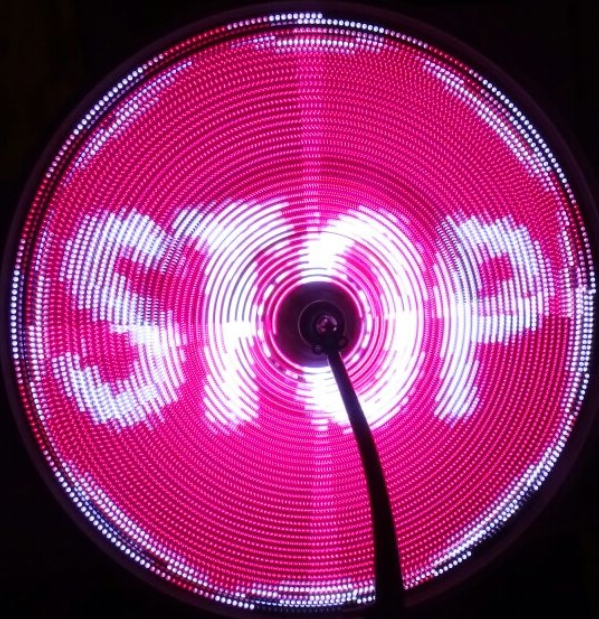
\includegraphics[width=7cm]{Stopschild.png}
	\caption{Skizze des Aufbaus}
\end{figure}
\subsection{Ergebnisdiskussion}
Nach einem ersten Start unseres Programmes haben wir festgestellt, dass der Raspberry Pi Zero, den wir wegen seiner geringen Größe und seinem kaum spürbaren Gewicht verwenden wollten, viel zu langsam ist, um ein hochauflösendes Bild darzustellen (siehe Abb. 7a). Der deutlich schnellere Raspberry Pi 3 erstellt hierbei einen viel besseres Bild (siehe Abb. 7b). Dies sieht man auch auf den beiden Bildern:
\begin{figure}[h]
\centering
\subfigure[Smily mit Raspberry Pi Zero]{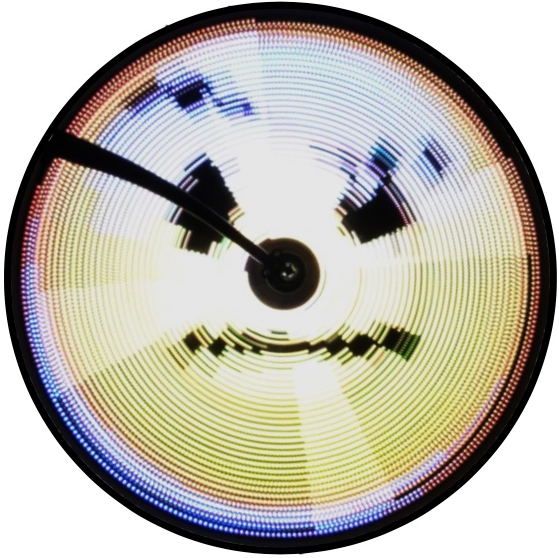
\includegraphics[width=5.0cm]{Smily0.png}} 
\subfigure[Smily mit Raspberry Pi 3]{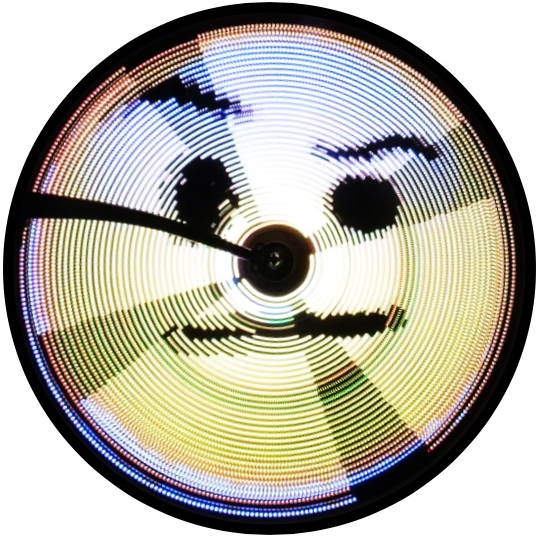
\includegraphics[width=5.0cm]{Smily3.png}}
\caption{Vergleich zwischen dem Raspberry Pi Zero und dem Raspberry Pi 3}
\end{figure}
\\Aus diesem Grund haben wir uns für den schnelleren Raspberry Pi 3 entschieden, den wir auch in Zukunft weiter verwenden werden. Der passt jedoch leider in keine für uns momentan verfügbare wasserdichte Verteilerbox. Daher ist das Speichendisplay momentan an einem Fahrrad noch nicht bei jedem Wetter einsetzbar.
\subsection{Geplante Verbesserungen}
Wir haben vor, unsere gesamte Apparatur wasserfest zu machen, damit man bei fast allen Wetterbedingungen mit dem Speichendisplay fahren kann. Im Laufe der weiteren Projektweiterentwicklung wollen wir die LED-Ansteuerung-Software durch selbstentwickelte Software ersetzen, um dieses Projekt ganz unser Eigen nennen zu können. Zum Steuern des Raspberry Pi planen wir den Raspberry Pi eine Website hosten zu lassen, auf die ein Nutzer über eine W-LAN Verbindung zum Raspberry Pi zugreifen und Bilder von seinem Endgerät auf den Raspberry Pi hochladen kann. Zusätzlich möchten wir insgesamt drei Magnetsensoren an das Rad montieren, um damit die Drehrichtung des Rades zu ermitteln. So können wir das Bild unabhängig von der Drehrichtung darstellen.
\section{Zusammenfassung}
Alles in allem ist das Speichendisplay eine interaktive, multifunktionale, kostengünstige und sicherheitsfördernde Anzeige, die jedoch noch kleine Kinderkrankheiten hat. Mit diesem Speichendisplay erhoffen wir uns, mehr Menschen zum sicheren Fahrradfahren, auch im Dunkeln, zu begeistern.
\section{Anhang}
\subsection{Quellen- und Literaturverzeichnis}
1)\\
http://www.pd-f.de/wp-content/uploads/kalins-pdf/singles/themenblatt-die-fahrradwelt-in- zahlen.pdf [Zugang am 03.01.2017, um 11:46 Uhr] \\
2)\\
http://www.monkeylectric.com/monkey\_light\_pro/ [Zugang am 10.01.2017, um 16:56 Uhr; Monkeylectric; Monkey Light Pro]\\
3)\\
https://learn.adafruit.com/neopixels-on-raspberry-pi/software [Zugang am 07.01.2017, um 17:08 Uhr; Toni DiCola; Adafruit-Neopixel-Library]\\
4)\\
http://www.elektronik-kompendium.de/sites/com/0902081.htm [Zugang am 9.1.2017, um 15:55 Uhr; Patrick Schnabel; USB-Stecker mit Steckerbelegung]\\
5)\\
https://github.com/python-pillow/Pillow [Zugang am 15.01.2017, um 11:37 Uhr; python- Pillow; Pillow]\\
6)\\
https://www.raspberrypi.org/downloads/raspbian/ [Zugang am 15.1.2017 um 11:54 Uhr; Raspberry Pi Foundation; Raspbian]\\
7)\\
https://i1.wp.com/www.novaspirit.com/wp-content/uploads/2016/10/wireing.jpg?ssl=1 [Zugang am 15.1.2017, um 09:38 Uhr; Novaspirit; USB Male Connector]\\
8)\\
https://www.raspberrypi.org/documentation/configuration/wireless/wireless-cli.md [Zugang am 15.1.2017, um 10:37 Uhr; Raspberry Pi Foundation; WLAN-Verbindung]\\
9)\\
https://www.raspberrypi.org/documentation/configuration/raspi-config.md [Zugang am 15.1.2017, um 10:14 Uhr; Alex Bradbury; Raspberry Pi Konfigurationseinstellungen]\\
10)\\
https://github.com/RubenHaag/Jufo\_Spokescreen [Zugang am 15.1.2017, um 11:59 Uhr; Ruben Haag; Projektordner]\\
11)\\
http://fritzing.org/download/ [Zugang am 18.01.2017, um 13:02 Uhr; Friends-of-Fritzing e.V.; Fritzing]\\
12)\\
https://www.conrad.de/de/abzweigkasten-l-x-b-x-h-75-x-40-x-37-mm-5229-licht-grau-ip54\\-629536.html? gclid=CPfQ7JrP29ECFcG7GwodF3UFtQ\&insert\_kz=VQ\&hk=SEM\&WT.srch=\\1\&WT.mc\_id=g oogle\_pla\&s\_kwcid=AL!222!3!173789970902!!!g!!\&ef\_id=WBpFUQAABUMWE\\wed: 20170124202753:s [Zugang am 26.01.2017, um 16:41 Uhr; Conrad Electronic SE; Platinenbox]\\
13)\\
https://www.notebooksbilliger.de/raspberry+pi+3+model+b+arm+cortex+a53/? nbb=pla.\\google\_\&wt\_cc2=913-0001\_Hardware\_257367\&gclid=CMeX0KL759ECFYGw7Qod 2q8CRQ [Zugang am 26.01.2017, um 16:45 Uhr; reichelt elektronik GmbH \& Co. KG; Raspberry Pi 3]\\
14)\\
http://www.ebay.de/itm/like/252355489432?lpid=106\&chn=ps\&ul\_noapp=true [Zugang am\\ 27.01.2017, um 15:29 Uhr; eBay Europe S.`a.r.l.; Kabel]\\
15)\\
http://www.ebay.de/itm/WS2812B-5050-RGB-144LED-1M-String-Strip-Lights-Addressable-\\ Waterproof-H3/111860633668? \_trksid=p2141725.c100338.m3726\&\_trkparms=aid\%3D222007\%\\26algo\%3DSIC.MBE\%26a o\%3D1\%26asc\%3D20150313114020\%26meid\%3D9977e8ae4b7e42c\\8990b9f5cc22f9914\% 26pid\%3D100338\%26rk\%3D1\%26rkt\%3D21\%26sd\%3D301963844528 [Zugang am 24.01.2017, um 18:47 Uhr; eBay Europe S.`a.r.l.; LED-Streifen]\\
16)\\
https://www.amazon.de/Anker-PowerCore-Powerbank-Ladeger"at-Smartphone/dp/ B01CU\\1EC6Y/ref=sr\_1\_1?s=ce- de\&ie=UTF8\&qid=1483383358\&sr=1-1\&keywords=akkupack [Zugang am 27.01.2017, um 16:41 Uhr; Amazon EU S.\`a r.l.; Powerbank]\\
17)\\
Paul Read, Mark-Paul Meyer: \glqq Restoration of motion picture film\grqq, Woburn, MA, USA 2000, S. 24\\
18)\\
Annette Lauber, Petra Schmalstieg: \glqq Band 2: Wahrnehemen und Beobachten\grqq, Stuttgart 2012, S. 9\\
19) \\
https://cdn-shop.adafruit.com/datasheets/WS2812B.pdf[Zugang am 20.2., um 8:00 Uhr; ; Dateblatt des LED-Streifens]
(Anmerkung: Die Zugangsdaten beziehen sich stets auf den Zeitpunkt des letzten Zugriffes)

\subsection{Danksagungen}
Wir vom Projekt \glqq Speichendisplay\grqq\ bedanken uns sehr bei der Fahrradwerkstatt der Holzkirche Lichterfelde für die Spende einer Fahrradgabel, ohne die unser Projekt nicht möglich gewesen wäre. Ebenfalls bedanken wir uns bei unserem Betreuer René Gorriz vom Paulsen-Gymnasium, der uns bei unserem Projekt tatkräftig unterstützt.
\newpage
\subsection{Kostenkalkulation und Materialliste}
\begin{figure}[h]
	\centering
	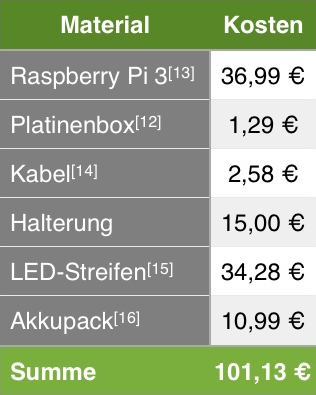
\includegraphics[width=4cm]{tab.png}
\end{figure}
\end{document}